% Options for packages loaded elsewhere
% Options for packages loaded elsewhere
\PassOptionsToPackage{unicode}{hyperref}
\PassOptionsToPackage{hyphens}{url}
%
\documentclass[
  ignorenonframetext,
  aspectratio=169,
]{beamer}
\newif\ifbibliography
\usepackage{pgfpages}
\setbeamertemplate{caption}[numbered]
\setbeamertemplate{caption label separator}{: }
\setbeamercolor{caption name}{fg=normal text.fg}
\beamertemplatenavigationsymbolsempty
% remove section numbering
\setbeamertemplate{part page}{
  \centering
  \begin{beamercolorbox}[sep=16pt,center]{part title}
    \usebeamerfont{part title}\insertpart\par
  \end{beamercolorbox}
}
\setbeamertemplate{section page}{
  \centering
  \begin{beamercolorbox}[sep=12pt,center]{section title}
    \usebeamerfont{section title}\insertsection\par
  \end{beamercolorbox}
}
\setbeamertemplate{subsection page}{
  \centering
  \begin{beamercolorbox}[sep=8pt,center]{subsection title}
    \usebeamerfont{subsection title}\insertsubsection\par
  \end{beamercolorbox}
}
% Prevent slide breaks in the middle of a paragraph
\widowpenalties 1 10000
\raggedbottom
\usepackage{iftex}
\ifPDFTeX
  \usepackage[T1]{fontenc}
  \usepackage[utf8]{inputenc}
  \usepackage{textcomp} % provide euro and other symbols
\else % if luatex or xetex
  \usepackage{unicode-math} % this also loads fontspec
  \defaultfontfeatures{Scale=MatchLowercase}
  \defaultfontfeatures[\rmfamily]{Ligatures=TeX,Scale=1}
\fi
\usepackage{lmodern}

\ifPDFTeX\else
  % xetex/luatex font selection
\fi
% Use upquote if available, for straight quotes in verbatim environments
\IfFileExists{upquote.sty}{\usepackage{upquote}}{}
\IfFileExists{microtype.sty}{% use microtype if available
  \usepackage[]{microtype}
  \UseMicrotypeSet[protrusion]{basicmath} % disable protrusion for tt fonts
}{}
\makeatletter
\@ifundefined{KOMAClassName}{% if non-KOMA class
  \IfFileExists{parskip.sty}{%
    \usepackage{parskip}
  }{% else
    \setlength{\parindent}{0pt}
    \setlength{\parskip}{6pt plus 2pt minus 1pt}}
}{% if KOMA class
  \KOMAoptions{parskip=half}}
\makeatother


\usepackage{longtable,booktabs,array}
\usepackage{calc} % for calculating minipage widths
\usepackage{caption}
% Make caption package work with longtable
\makeatletter
\def\fnum@table{\tablename~\thetable}
\makeatother
\usepackage{graphicx}
\makeatletter
\newsavebox\pandoc@box
\newcommand*\pandocbounded[1]{% scales image to fit in text height/width
  \sbox\pandoc@box{#1}%
  \Gscale@div\@tempa{\textheight}{\dimexpr\ht\pandoc@box+\dp\pandoc@box\relax}%
  \Gscale@div\@tempb{\linewidth}{\wd\pandoc@box}%
  \ifdim\@tempb\p@<\@tempa\p@\let\@tempa\@tempb\fi% select the smaller of both
  \ifdim\@tempa\p@<\p@\scalebox{\@tempa}{\usebox\pandoc@box}%
  \else\usebox{\pandoc@box}%
  \fi%
}
% Set default figure placement to htbp
\def\fps@figure{htbp}
\makeatother


% definitions for citeproc citations
\NewDocumentCommand\citeproctext{}{}
\NewDocumentCommand\citeproc{mm}{%
  \begingroup\def\citeproctext{#2}\cite{#1}\endgroup}
\makeatletter
 % allow citations to break across lines
 \let\@cite@ofmt\@firstofone
 % avoid brackets around text for \cite:
 \def\@biblabel#1{}
 \def\@cite#1#2{{#1\if@tempswa , #2\fi}}
\makeatother
\newlength{\cslhangindent}
\setlength{\cslhangindent}{1.5em}
\newlength{\csllabelwidth}
\setlength{\csllabelwidth}{3em}
\newenvironment{CSLReferences}[2] % #1 hanging-indent, #2 entry-spacing
 {\begin{list}{}{%
  \setlength{\itemindent}{0pt}
  \setlength{\leftmargin}{0pt}
  \setlength{\parsep}{0pt}
  % turn on hanging indent if param 1 is 1
  \ifodd #1
   \setlength{\leftmargin}{\cslhangindent}
   \setlength{\itemindent}{-1\cslhangindent}
  \fi
  % set entry spacing
  \setlength{\itemsep}{#2\baselineskip}}}
 {\end{list}}
\usepackage{calc}
\newcommand{\CSLBlock}[1]{\hfill\break\parbox[t]{\linewidth}{\strut\ignorespaces#1\strut}}
\newcommand{\CSLLeftMargin}[1]{\parbox[t]{\csllabelwidth}{\strut#1\strut}}
\newcommand{\CSLRightInline}[1]{\parbox[t]{\linewidth - \csllabelwidth}{\strut#1\strut}}
\newcommand{\CSLIndent}[1]{\hspace{\cslhangindent}#1}



\setlength{\emergencystretch}{3em} % prevent overfull lines

\providecommand{\tightlist}{%
  \setlength{\itemsep}{0pt}\setlength{\parskip}{0pt}}



 


% WHU beamer theme (16:9) - v3
% Usage: \input{materials/beamer_theme_16x9.sty}
\ProvidesFile{00_theme.sty}[2026/03/13 WHU beamer theme v3]

\mode<presentation>

% ── Package dependencies ────────────────────────────────────────
\RequirePackage{tikz}
\usetikzlibrary{calc,positioning,arrows.meta,shapes.geometric,fit,backgrounds}
\RequirePackage{etoolbox}
\RequirePackage{ifxetex}
\RequirePackage{booktabs}
\RequirePackage{tabularx}
\RequirePackage{ragged2e}
\RequirePackage{amsmath,amssymb}
\RequirePackage{appendixnumberbeamer}

% ── Fonts ───────────────────────────────────────────────────────
\RequirePackage{lmodern}
\RequirePackage[T1]{fontenc}
\RequirePackage[utf8]{inputenc}

% ── Colors ──────────────────────────────────────────────────────
\definecolor{whu_blue}{RGB}{5,70,150}
\definecolor{whu_lightblue}{RGB}{0,165,220}
\definecolor{whu_silvergray}{RGB}{230,235,240}
\definecolor{whu_anthracite}{RGB}{80,84,89}
\definecolor{whu_darkgray}{RGB}{60,60,60}
\definecolor{whu_accent_green}{RGB}{0,128,85}
\definecolor{whu_accent_red}{RGB}{180,40,40}
\definecolor{whu_accent_orange}{RGB}{210,120,20}
\definecolor{whu_lightgreen}{RGB}{230,245,235}
\definecolor{whu_lightred}{RGB}{250,235,235}

% ── Global beamer color setup ───────────────────────────────────
\setbeamercolor*{title}{fg=whu_blue}
\setbeamercolor*{subtitle}{fg=whu_blue}
\setbeamercolor*{title page header}{fg=whu_blue}
\setbeamercolor*{author}{fg=whu_blue}
\setbeamercolor*{institute}{fg=white}
\setbeamercolor*{date}{fg=white}
\setbeamercolor*{normal text}{fg=black}

% Items
\setbeamercolor*{item}{fg=whu_blue}
\setbeamercolor*{itemize item}{fg=whu_blue}
\setbeamercolor*{itemize subitem}{parent=itemize item}
\setbeamercolor*{itemize subsubitem}{parent=itemize item}
\setbeamercolor*{enumerate item}{fg=whu_blue}
\setbeamercolor*{enumerate subitem}{parent=enumerate item}
\setbeamercolor*{description item}{fg=whu_blue}
\setbeamerfont{description item}{series=\bfseries}

\setbeamercolor*{frametitle}{fg=whu_blue}
\setbeamercolor*{page number in head/foot}{fg=whu_blue}

% Blocks
\setbeamercolor*{block title}{fg=whu_blue,bg=whu_silvergray}
\setbeamercolor*{block body}{fg=black,bg=whu_silvergray!30}
\setbeamercolor*{block title alerted}{fg=white,bg=whu_accent_red}
\setbeamercolor*{block body alerted}{fg=black,bg=whu_lightred}
\setbeamercolor*{block title example}{fg=white,bg=whu_accent_green}
\setbeamercolor*{block body example}{fg=black,bg=whu_lightgreen}

% ── Font sizes ──────────────────────────────────────────────────
\setbeamerfont{title}{size=\LARGE,series=\bfseries}
\setbeamerfont{subtitle}{size=\large}
\setbeamerfont{frametitle}{size=\large,series=\bfseries}
\setbeamerfont{framesubtitle}{size=\small}
\setbeamerfont{block title}{size=\normalsize,series=\bfseries}
\setbeamerfont{footnote}{size=\tiny}

% ── Hyperlinks ──────────────────────────────────────────────────
\hypersetup{colorlinks=true,urlcolor=whu_lightblue,linkcolor=whu_lightblue}

% ── Navigation / footline ──────────────────────────────────────
\setbeamertemplate{navigation symbols}{}
\setbeamertemplate{blocks}[rounded][shadow=false]
\setbeamertemplate{footline}[frame number]

% ── Background ──────────────────────────────────────────────────
\setbeamertemplate{background}{%
  \begin{tikzpicture}
    \useasboundingbox (0,0) rectangle(\the\paperwidth,\the\paperheight);
    \ifnum\thepage=1\relax
      \fill[white] (0,0) rectangle(\the\paperwidth,\the\paperheight);
      \fill[whu_blue!60] (0,0) rectangle(1.5,1.9);
      \fill[whu_blue] (1.6,0) rectangle(\the\paperwidth,1.9);
      \node[anchor=west,text=white,font=\small] at (1.7,1.18) {\insertinstitute};
      \node[anchor=west,text=white,font=\small] at (1.7,0.6) {\insertdate};
    \else
      \fill[white] (0,0) rectangle(\the\paperwidth,\the\paperheight);
    \fi
  \end{tikzpicture}%
}

% ── Title page ──────────────────────────────────────────────────
\defbeamertemplate*{title page}{whu266}[1][]
{%
  \vskip.5cm
  
\includegraphics[keepaspectratio,height=1.5cm]{materials/00_whu_logo.png}
  \vskip1.5cm
  \begin{beamercolorbox}[wd=12cm,leftskip=0.6cm,#1]{title page header}
    \usebeamerfont{title}\inserttitle\par
    \usebeamerfont{subtitle}\insertsubtitle\par
  \end{beamercolorbox}
  \vskip1.5cm
  \begin{beamercolorbox}[wd=12cm,leftskip=0.6cm,sep=1pt,#1]{author}
    \usebeamerfont{author}\insertauthor
  \end{beamercolorbox}
  % institute + date are drawn onto the bottom bar by the page-1 background
  % template (so the date is never clipped). Reserve their original vertical
  % footprint here so the title and author keep their previous position.
  \vskip2.05cm
  \vfil
}
\setbeamertemplate{title page}[whu266]

% ── Items / ToC ─────────────────────────────────────────────────
\setbeamertemplate{items}[square]
\setbeamertemplate{sections/subsections in toc}[square]

% ── Frame title ─────────────────────────────────────────────────
\makeatletter
\defbeamertemplate*{frametitle}{whu266}[1][]
{%
  \vskip0.6cm%
  \begin{beamercolorbox}[wd=\paperwidth,ht=0.5cm]{frametitle}
    \begin{tikzpicture}
      \useasboundingbox[fill=white] (0,0) rectangle(\the\paperwidth,0.5);
      \fill[whu_blue!60] (0,0) rectangle(1.5,1.2);
      \fill[whu_blue] (1.6,0) rectangle(\the\paperwidth,1.2);
      \ifx\insertframesubtitle\@empty%
        \node[anchor=west,white,font=\large] at (1.7,0.6) {\insertframetitle};
      \else%
        \node[anchor=west,white,font=\large] at (1.7,0.75) {\insertframetitle};
        \node[anchor=west,white,font=\small] at (1.7,0.35) {\insertframesubtitle};
      \fi
    \end{tikzpicture}
  \end{beamercolorbox}
}
\makeatother
\setbeamertemplate{frametitle}[whu266]

% ═════════════════════════════════════════════════════════════════
% UTILITY MACROS - Full toolkit for varied slide layouts
% ═════════════════════════════════════════════════════════════════

% ── Section divider slide ───────────────────────────────────────
% Usage: \sectionslide{Section Title}
\newcommand{\sectionslide}[1]{%
  \begin{frame}[plain]
    \vfill
    \hspace*{-\dimexpr(\paperwidth-\textwidth)/2\relax}%
    \makebox[0pt][l]{%
    \begin{tikzpicture}
      \useasboundingbox (0,0) rectangle(\the\paperwidth,3);
      \fill[whu_blue!60] (0,1.0) rectangle(1.5,2.2);
      \fill[whu_blue] (1.6,1.0) rectangle(\the\paperwidth,2.2);
      \node[anchor=west,white,font=\LARGE\bfseries] at (1.7,1.6) {#1};
    \end{tikzpicture}%
    }
    \vfill
  \end{frame}%
}

% ── Highlight box (gray background) ────────────────────────────
% Usage: \highlightbox{Key definition or important text.}
\newcommand{\highlightbox}[1]{%
  \begin{tikzpicture}
    \node[fill=whu_silvergray,rounded corners=3pt,inner sep=8pt,
          text width=\linewidth-20pt] {#1};
  \end{tikzpicture}%
}

% ── Source citation at bottom of slide ─────────────────────────
% Usage: \source{Author (Year)}
\newcommand{\source}[1]{%
  \vfill
  {\usebeamerfont{footnote}\textcolor{whu_anthracite}{Source: #1}}%
}

% ── AGENTS.md rule tag at bottom of slide ──────────────────────
% Usage: \agentrule{Never modify the raw data in 0\_data/. It is read-only.}
\newcommand{\agentrule}[1]{%
  \vfill
  {\usebeamerfont{footnote}\itshape\textcolor{whu_anthracite}{AGENTS.md: ``#1''}}%
}

% ── Single stat callout ────────────────────────────────────────
% Usage: \statcallout{42\%}{of firms use AI in forecasting}
\newcommand{\statcallout}[2]{%
  \begin{center}
    {\fontsize{42}{48}\selectfont\textcolor{whu_blue}{\textbf{#1}}}\\[4pt]
    {\large\textcolor{whu_anthracite}{#2}}
  \end{center}%
}

% ── Double stat callout (side-by-side numbers) ─────────────────
% Usage: \doublestat{73\%}{use quantitative}{12\%}{use mixed methods}
\newcommand{\doublestat}[4]{%
  \begin{columns}[c]
    \begin{column}{0.48\textwidth}
      \begin{center}
        {\fontsize{38}{44}\selectfont\textcolor{whu_blue}{\textbf{#1}}}\\[4pt]
        {\normalsize\textcolor{whu_anthracite}{#2}}
      \end{center}
    \end{column}
    \begin{column}{0.48\textwidth}
      \begin{center}
        {\fontsize{38}{44}\selectfont\textcolor{whu_accent_green}{\textbf{#3}}}\\[4pt]
        {\normalsize\textcolor{whu_anthracite}{#4}}
      \end{center}
    \end{column}
  \end{columns}%
}

% ── Discussion prompt box ──────────────────────────────────────
%Usage: \discussionprompt{What would you do if...?}
% \newcommand{\discussionprompt}[1]{%
%   \begin{tikzpicture}
%     \node[fill=whu_blue!10,draw=whu_blue,rounded corners=4pt,
%           inner sep=10pt,text width=\linewidth-24pt,
%           font=\large\itshape] {#1};
%   \end{tikzpicture}%
% }

\newcommand{\discussionprompt}[1]{%
  \begin{tikzpicture}
    \node[fill=whu_blue!8,draw=whu_blue,rounded corners=4pt,
          inner sep=10pt,text width=\linewidth-24pt] {#1};
  \end{tikzpicture}%
}

% ── How box ───────────────────────────────────────────
% Usage: \how{The main point the student should remember.}
\newcommand{\how}[1]{%
  \begin{tikzpicture}
    \node[fill=whu_blue!8,draw=whu_blue,line width=0.8pt,
          rounded corners=4pt,inner sep=10pt,
          text width=\linewidth-24pt] {%
      {\textbf{\textcolor{whu_blue}{How?}} #1}%
    };
  \end{tikzpicture}%
}

% ── Key takeaway box ───────────────────────────────────────────
% Usage: \takeaway{The main point the student should remember.}
\newcommand{\takeaway}[1]{%
  \begin{tikzpicture}
    \node[fill=whu_blue!8,draw=whu_blue,line width=0.8pt,
          rounded corners=4pt,inner sep=10pt,
          text width=\linewidth-24pt] {%
      {\textbf{\textcolor{whu_blue}{Key takeaway:}} #1}%
    };
  \end{tikzpicture}%
}

% ── Quote / Epigraph ──────────────────────────────────────────
% Usage: \epigraphslide{The quote text here.}{Author Name}
\newcommand{\epigraphslide}[2]{%
  \vfill
  \begin{center}
    \begin{minipage}{0.8\linewidth}
      {\Large\itshape\textcolor{whu_anthracite}{``#1''}}\\[10pt]
      \hfill{\normalsize\textcolor{whu_blue}{\textbf{--- #2}}}
    \end{minipage}
  \end{center}
  \vfill
}

% ── Horizontal process flow ────────────────────────────────────
% Usage: \process{Step 1,Step 2,Step 3,Step 4}
% Usage: \process{Step 1/whu_lightblue,Step 2,Step 3}
\newcommand{\process}[1]{%
  \begin{center}
  \begin{tikzpicture}[
    node distance=0.3cm,
    flowstep/.style={rectangle,rounded corners=3pt,fill=whu_blue,
                 text=white,font=\small\bfseries,
                 minimum height=0.9cm,minimum width=2.4cm,
                 text width=2.2cm,align=center},
    arr/.style={-{Stealth[length=5pt]},line width=1.2pt,whu_lightblue}
  ]
    \foreach \s/\c [count=\i] in {#1} {
      \edef\nodecolor{\c}%
      \edef\nodelabel{\s}%
      \ifx\nodecolor\nodelabel\def\nodecolor{whu_blue}\fi%
      \ifnum\i=1
        \node[flowstep,fill=\nodecolor] (s\i) {\s};
      \else
        \pgfmathtruncatemacro{\prev}{\i - 1}
        \node[flowstep,fill=\nodecolor,right=of s\prev] (s\i) {\s};
        \draw[arr] (s\prev) -- (s\i);
      \fi
    }
  \end{tikzpicture}
  \end{center}%
}

% ── Circular process cycle ─────────────────────────────────────
% Usage: \processcycle{Step 1,Step 2,Step 3,Step 4}
\newcommand{\processcycle}[1]{%
  \xdef\totalsteps{0}%
  \foreach \s/\c in {#1} {%
    \pgfmathtruncatemacro{\tmp}{\totalsteps+1}%
    \xdef\totalsteps{\tmp}%
  }%
  \begin{center}
  \begin{tikzpicture}[
    flowstep/.style={rectangle,rounded corners=3pt,fill=whu_blue,
                 text=white,font=\small\bfseries,
                 minimum height=0.9cm,minimum width=2.4cm,
                 text width=2.2cm,align=center},
    arr/.style={-{Stealth[length=5pt]},line width=1.2pt,whu_lightblue}
  ]
    \foreach \s/\c [count=\i] in {#1} {%
      \edef\nodecolor{\c}%
      \edef\nodelabel{\s}%
      \ifx\nodecolor\nodelabel\def\nodecolor{whu_blue}\fi%
      \pgfmathsetmacro{\angle}{90 - (\i-1)*360/\totalsteps}%
      \node[flowstep,fill=\nodecolor] (s\i) at (\angle:3cm) {\s};%
    }
    \foreach \s/\c [count=\i] in {#1} {%
      \pgfmathtruncatemacro{\next}{int(mod(\i,\totalsteps)+1)}%
      \draw[arr] (s\i) -- (s\next);%
    }
  \end{tikzpicture}
  \end{center}%
}

% ── Numbered step label (inline) ──────────────────────────────
% Usage: \stepnum{1} First step description.
\newcommand{\stepnum}[1]{%
  \tikz[baseline=(num.base)]{
    \node[fill=whu_blue,text=white,circle,inner sep=2pt,
          font=\small\bfseries,minimum size=0.55cm] (num) {#1};
  }%
}

% ── Comparison marks ──────────────────────────────────────────
% Usage: \cmark and \xmark in tables and lists
\newcommand{\cmark}{\textcolor{whu_accent_green}{\textbf{\checkmark}}}
\providecommand{\xmark}{\textcolor{whu_accent_red}{\textbf{\texttimes}}}

\mode<all>
\usepackage{wrapfig}
\usepackage{subcaption}
\usepackage{newunicodechar}
\newunicodechar{š}{\v{s}}
\AtBeginSection[]{\sectionslide{\insertsectionhead}}
\makeatletter
\@ifpackageloaded{caption}{}{\usepackage{caption}}
\AtBeginDocument{%
\ifdefined\contentsname
  \renewcommand*\contentsname{Table of contents}
\else
  \newcommand\contentsname{Table of contents}
\fi
\ifdefined\listfigurename
  \renewcommand*\listfigurename{List of Figures}
\else
  \newcommand\listfigurename{List of Figures}
\fi
\ifdefined\listtablename
  \renewcommand*\listtablename{List of Tables}
\else
  \newcommand\listtablename{List of Tables}
\fi
\ifdefined\figurename
  \renewcommand*\figurename{Figure}
\else
  \newcommand\figurename{Figure}
\fi
\ifdefined\tablename
  \renewcommand*\tablename{Table}
\else
  \newcommand\tablename{Table}
\fi
}
\@ifpackageloaded{float}{}{\usepackage{float}}
\floatstyle{ruled}
\@ifundefined{c@chapter}{\newfloat{codelisting}{h}{lop}}{\newfloat{codelisting}{h}{lop}[chapter]}
\floatname{codelisting}{Listing}
\newcommand*\listoflistings{\listof{codelisting}{List of Listings}}
\makeatother
\makeatletter
\makeatother
\makeatletter
\@ifpackageloaded{caption}{}{\usepackage{caption}}
\@ifpackageloaded{subcaption}{}{\usepackage{subcaption}}
\makeatother

\usepackage{bookmark}
\IfFileExists{xurl.sty}{\usepackage{xurl}}{} % add URL line breaks if available
\urlstyle{same}
\hypersetup{
  pdftitle={From Raw Data to Finished Paper: Building a Reproducible Research Pipeline},
  pdfauthor={Dr.~Victor van Pelt},
  hidelinks,
  pdfcreator={LaTeX via pandoc}}


\title{From Raw Data to Finished Paper: Building a Reproducible Research
Pipeline}
\subtitle{Doctoral Orientation Week}
\author{Dr.~Victor van Pelt}
\date{July 15, 2026}
\institute{WHU -- Otto Beisheim School of Management}

\begin{document}
\frame{\titlepage}


\begin{frame}{Opening Question}
\phantomsection\label{opening-question}
Let's say you wrote a research paper and your laptop died. How long
would it take you to reproduce your analyses with a new laptop?

\begin{enumerate}
\item
  Less than one hour (easy!)
\item
  Between one hour and a day (It's possible but painful)
\item
  More than one day (I'd be stuck)
\end{enumerate}
\end{frame}

\begin{frame}{Why should YOU care about Data Management?}
\phantomsection\label{why-should-you-care-about-data-management}
\centering

Storing data, code, and analyses can quickly turn into a mess:

\begin{center}
\includegraphics[width =0.6\textwidth]{"images/pic2.png"} \\
\end{center}
\end{frame}

\begin{frame}{Why should YOU care about Data Management?}
\phantomsection\label{why-should-you-care-about-data-management-1}
\begin{center}
Story Time!
\bigbreak
\includegraphics[width =0.50\textwidth]{"images/figure3.jpg"} \\
\end{center}
\end{frame}

\begin{frame}{But there is more at stake!}
\phantomsection\label{but-there-is-more-at-stake}
\centering

In 2019, \emph{Management Science} introduced a Data and Code Disclosure
Policy:

\emph{``Authors of accepted papers\ldots{} must provide\ldots{} the
data, programs, and other details of the experiment and computations
sufficient to permit replication.''}

A 2024 study examined nearly 500 articles published before and after
this policy was introduced to see if the results could, in fact, be
reproduced (Fišar et al. 2024).

\textbf{What share of these articles do you think were largely
reproducible?}
\end{frame}

\begin{frame}{But there is more at stake!}
\phantomsection\label{but-there-is-more-at-stake-1}
\begin{center}
\includegraphics[width =0.60\textwidth]{"images/figure2.png"} \\
\end{center}

\centering

Across all articles under the new policy, 68\% could be reproduced. When
data and software were accessible, over 95\% could (Fišar et al. 2024)
\end{frame}

\begin{frame}{But there is more at stake!}
\phantomsection\label{but-there-is-more-at-stake-2}
\centering

\begin{itemize}
\tightlist
\item
  Even under the policy, nearly one in three papers fails the
  reproducibility test.
\item
  Before the policy, it was worse: only 12\% of articles shared any
  materials at all.
\item
  This is why good data and code management is not only a ``nice to
  have.''
\item
  It's also essential for credible research and for us to trust the
  insights it produces.
\item
  But this does not just depend on how professors manage their data and
  code.
\item
  It all starts with:
\end{itemize}

\begin{center}
\includegraphics[width =0.20\textwidth]{"images/you.png"} \\
\end{center}
\end{frame}

\begin{frame}{The main goals of this session:}
\phantomsection\label{the-main-goals-of-this-session}
\begin{itemize}
\tightlist
\item
  Share a few basic principles, techniques, and tools. Inspired by:

  \begin{itemize}
  \tightlist
  \item
    \href{https://web.stanford.edu/~gentzkow/research/CodeAndData.pdf}{\textbf{Code
    and Data for the Social Sciences} (Gentzkow and Shapiro)}
  \item
    \href{https://medium.com/data-science/how-to-keep-your-research-projects-organized-part-1-folder-structure-10bd56034d3a}{\textbf{How
    to keep your research projects organized} (de Kok)}
  \item
    \href{https://journals.plos.org/ploscompbiol/article?id=10.1371/journal.pcbi.1005510}{\textbf{Good
    Enough Practices in Scientific Computing} (Wilson et al.)}
  \item
    My own mistakes and personal experience
  \end{itemize}
\item
  Let's make this interactive: Interrupt, ask questions, and tell me
  about your experience.
\item
  Disclaimer: Largely through the lens of a quantitative researcher.
\item
  All materials for this talk are available:
  \href{https://github.com/victorvanpelt/research_pipeline_example}{\textbf{Example
  Files}} and
  \href{https://tinyurl.com/datamanagementslides}{\textbf{Slides}}
\end{itemize}
\end{frame}

\begin{frame}{What will we cover in this session?}
\phantomsection\label{what-will-we-cover-in-this-session}
\begin{enumerate}
\item
  Directory structure: How to organize your research project
\item
  Version control: Using Git and repositories (example using GitHub)
\item
  Integrating multiple languages: Example using Quarto
\item
  AI agents and systems: Using them without losing reproducibility, plus
  advice for your own setup
\end{enumerate}
\end{frame}

\section{1. Directory Structure}\label{directory-structure}

\begin{frame}{1. Directory Structure: Fundamental Principles}
\phantomsection\label{directory-structure-fundamental-principles}
\centering

Following principles is critical, especially for projects with lots of
data and code:

\begin{itemize}
\tightlist
\item
  Anyone can run the code anywhere and anytime, regardless of location.
\item
  Anyone can understand the code and data without much effort.
\item
  Anyone can update the code on the spot without breaking it (dynamic
  coding).
\end{itemize}
\end{frame}

\begin{frame}{1. Directory Structure: Structure the flow}
\phantomsection\label{directory-structure-structure-the-flow}
\begin{itemize}
\tightlist
\item
  Use a flow-inspired folder structure:

  \begin{itemize}
  \tightlist
  \item
    E.g., formatting files -\textgreater{} generating variables
    -\textgreater{} conducting analyses -\textgreater{} generating
    output.
  \end{itemize}
\item
  Leave the raw data untouched: You load it and use it to produce
  output:

  \begin{itemize}
  \tightlist
  \item
    E.g., raw data files -\textgreater{} input files -\textgreater{}
    process files -\textgreater{} output files.
  \end{itemize}
\item
  Use relative paths (e.g., ``\emph{../0\_data/data.csv}'') and not
  direct paths (e.g.,
  ``\emph{C:/user{[}name{]}/Documents/research/project\_1/0\_data/data.csv}'').
\end{itemize}

\highlightbox{Anyone should be able to delete everything except the raw data and the code, and rebuild your whole project.}
\end{frame}

\begin{frame}{1. Directory Structure: Code so others can run it}
\phantomsection\label{directory-structure-code-so-others-can-run-it}
\begin{itemize}
\tightlist
\item
  Make your code deterministic: set a seed for random and stochastic
  processes.
\item
  Pin your environment: ``\emph{version}'' in Stata, \emph{renv} in R.
\item
  Use plenty of comments to explain what the code is doing.
\item
  Be as descriptive as you can in folder and file names.
\item
  Use environment variables for credentials and software paths.
\item
  Follow a template for a research pipeline
  (\href{https://www.projecttier.org/tier-protocol/protocol-4-0/}{\textbf{TIER
  Protocol}}); the example repository follows its concept.

  \begin{itemize}
  \tightlist
  \item
    E.g., a codebook (``\emph{0\_data/codebook.md}'') defines each
    variable and the data's origin.
  \end{itemize}
\end{itemize}
\end{frame}

\begin{frame}{1. Directory Structure: A simple starting point}
\phantomsection\label{directory-structure-a-simple-starting-point}
\begin{center}
\includegraphics[width =0.75\textwidth]{"images/figure4.png"}
\end{center}
\end{frame}

\begin{frame}{1. Directory Structure: Additional folders}
\phantomsection\label{directory-structure-additional-folders}
\begin{center}

\includegraphics[width =0.75\textwidth]{"images/figure5.png"}
\end{center}
\end{frame}

\begin{frame}{1. Directory Structure: A working example}
\phantomsection\label{directory-structure-a-working-example}
\centering

Let's take a closer look at how this works in practice (using Stata, R,
and Quarto):

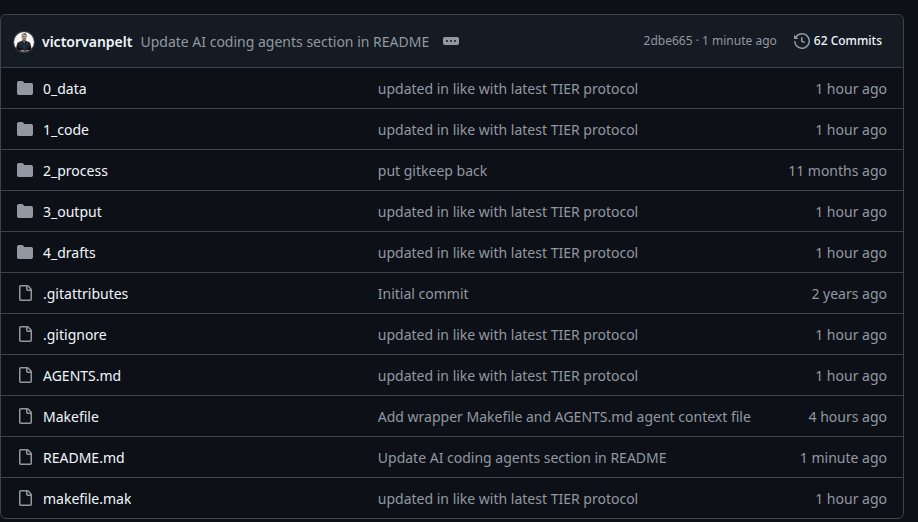
\includegraphics[width=3.02083in,height=\textheight,keepaspectratio]{images/paste-7.png}

\href{https://github.com/victorvanpelt/research_pipeline_example}{\textbf{Clone
this repository!}}

\href{https://github.com/victorvanpelt/research_pipeline_example}{\textbf{github.com/victorvanpelt/research\_pipeline\_example}}

The repository also ships a rulebook for AI agents
(``\emph{AGENTS.md}''): more in chapter 4.
\end{frame}

\begin{frame}{1. Directory Structure: Stata do-file under ``1\_code/''}
\phantomsection\label{directory-structure-stata-do-file-under-1_code}
\centering

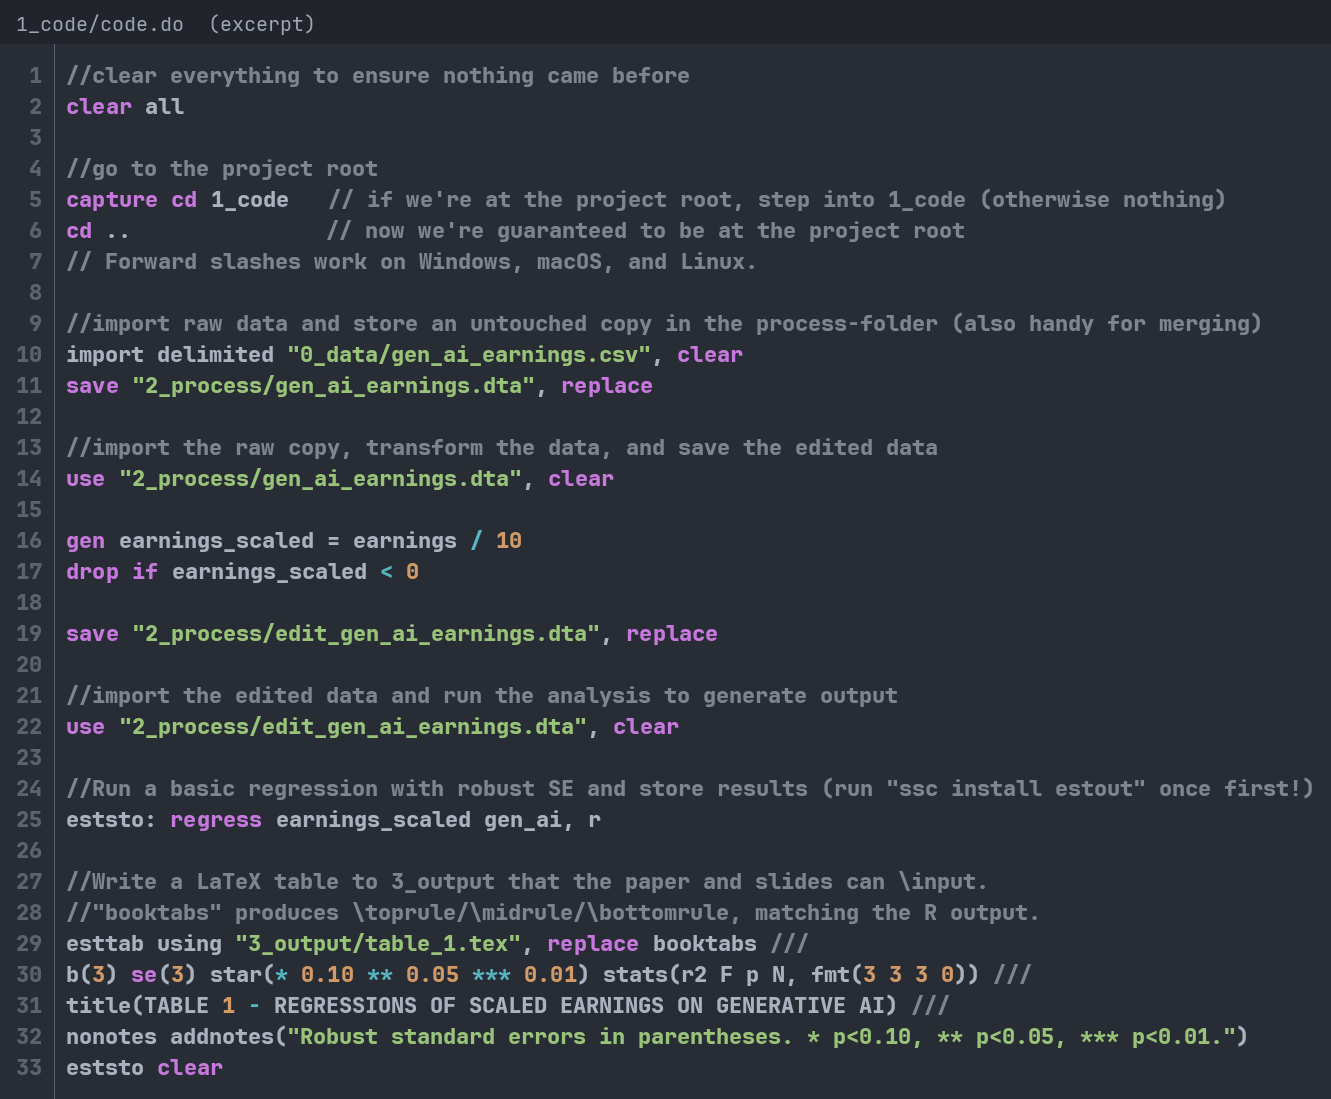
\includegraphics[width=\linewidth,height=2.44792in,keepaspectratio]{images/paste-4.png}

The same analysis also ships in R (``\emph{code.r}'') and Quarto
(``\emph{code.qmd}'')
\end{frame}

\begin{frame}{1. Directory Structure: Reproducing all results instantly}
\phantomsection\label{directory-structure-reproducing-all-results-instantly}
How would you reproduce all results of your current project?

\begin{enumerate}
\item
  One command rebuilds everything (a makefile or master script)
\item
  A script per step, run by hand in the right order
\item
  Point and click, from memory
\end{enumerate}
\end{frame}

\begin{frame}{1. Directory Structure: makefile.mak in root}
\phantomsection\label{directory-structure-makefile.mak-in-root}
\centering

A makefile states which outputs depend on which code and data, and how
to rebuild them \begin{center}
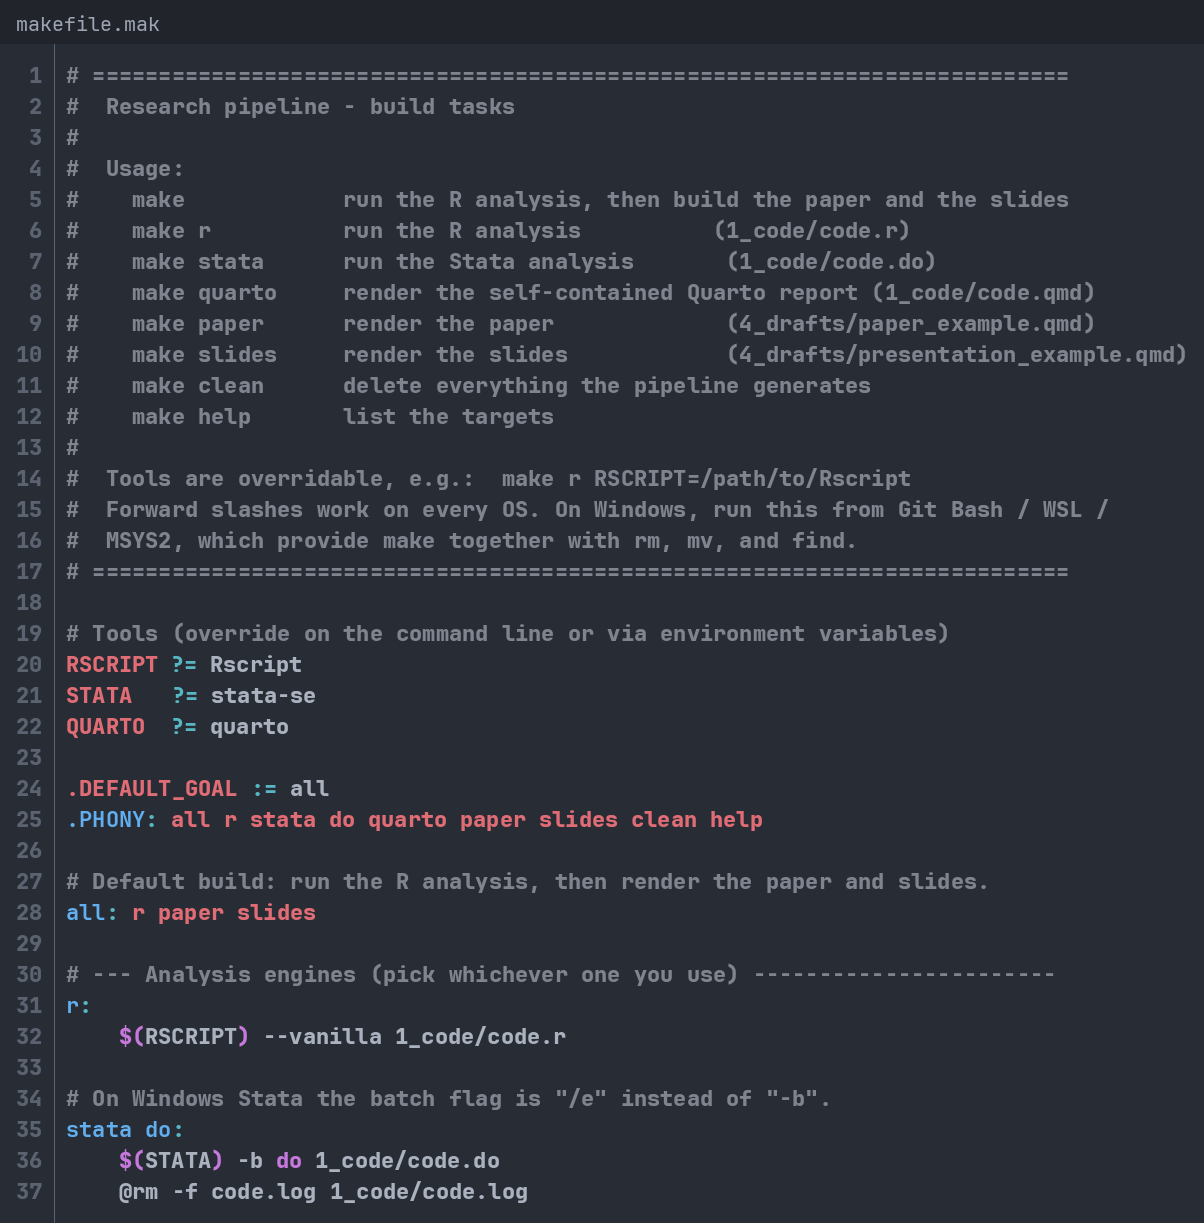
\includegraphics[width=\linewidth,height=2.44792in,keepaspectratio]{images/paste-19.png}
\end{center}
\end{frame}

\begin{frame}{1. Directory Structure: makefile.mak in root}
\phantomsection\label{directory-structure-makefile.mak-in-root-1}
\centering

You run ``\emph{make}'' in the CLI to rebuild everything, or a single
step with ``\emph{make r}'', ``\emph{make stata}'', ``\emph{make
appendix}'', ``\emph{make paper}'', or ``\emph{make slides}''
\begin{center}
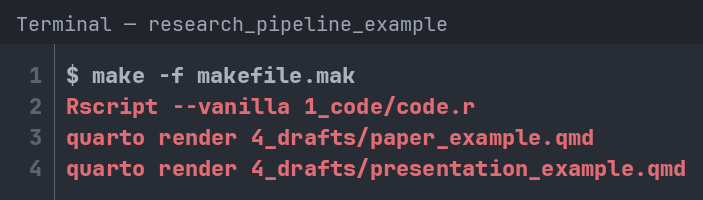
\includegraphics[width=\linewidth,height=1.30208in,keepaspectratio]{images/paste-16.png}
\end{center}
\end{frame}

\begin{frame}{1. Directory Structure: Is your code slow?}
\phantomsection\label{directory-structure-is-your-code-slow}
\begin{itemize}
\tightlist
\item
  Does your code:

  \begin{itemize}
  \tightlist
  \item
    Take a long time to run?
  \item
    Require too much memory?
  \end{itemize}
\item
  Ask your supervisor for a new laptop.
\item
  Otherwise, consider looking into running your code remotely:

  \begin{itemize}
  \tightlist
  \item
    A ``supercomputer,'' ``grid,'' or ``server'' allows you to run your
    code using much more powerful hardware.
  \item
    Ask about your school's research computing services.
  \end{itemize}
\end{itemize}
\end{frame}

\section{2. Version Control}\label{version-control}

\begin{frame}{2. Version control: Opening question}
\phantomsection\label{version-control-opening-question}
\centering

Whose folders look something like this?

\begin{center}
\includegraphics[width =0.3\textwidth]{"images/pic1.png"} \\
\end{center}
\end{frame}

\begin{frame}{2. Version control}
\phantomsection\label{version-control-1}
\centering

Version control is a system that records changes to a file or set of
files over time so that you can recall specific versions later.

\begin{center}
\includegraphics[width=\linewidth,height=1.82292in,keepaspectratio]{images/section_2.png}
\end{center}
\end{frame}

\begin{frame}{2. Version control: How to use version control}
\phantomsection\label{version-control-how-to-use-version-control}
\begin{itemize}
\tightlist
\item
  Many cloud services have some forms of version control (e.g., Dropbox
  and OneDrive), but they can be too simplistic and unreliable.
\item
  The most widely used software is called
  \href{https://git-scm.com/}{\textbf{git}}
\item
  You can run \href{https://git-scm.com/}{\textbf{git}} locally using
  the command line (CLI), but it is easier to use an online provider.
\item
  Saving your version control online reduces the likelihood you lose
  stuff.
\item
  Three major \href{https://git-scm.com/}{\textbf{git}} providers:

  \begin{itemize}
  \tightlist
  \item
    GitHub --\textgreater{} The best choice!
  \item
    Bitbucket
  \item
    GitLab
  \item
    (EU nonprofit alternative: Codeberg)
  \end{itemize}
\end{itemize}
\end{frame}

\begin{frame}{2. Version control: What is GitHub?}
\phantomsection\label{version-control-what-is-github}
\begin{itemize}
\tightlist
\item
  GitHub hosts your git repositories online and adds collaboration tools
  around them.
\item
  Why use it?

  \begin{itemize}
  \tightlist
  \item
    Clean and easy-to-use interface
  \item
    Works with any language and file type
  \item
    GitHub Desktop application is very simple and convenient
  \end{itemize}
\item
  Bonus feature: you can use GitHub Pages to host your website for free!
  See mine
  \href{https://www.victorvanpelt.com}{\textbf{www.victorvanpelt.com}}
\end{itemize}
\end{frame}

\begin{frame}{2. Version control: GitHub Education}
\phantomsection\label{version-control-github-education}
\centering

As a verified student, you get GitHub Pro and the Student Developer Pack
for free \href{https://education.github.com/pack}{\textbf{here}}.
\begin{center}
\includegraphics[width=\linewidth,height=2.34375in,keepaspectratio]{images/paste-14.png}
\end{center}
\end{frame}

\begin{frame}{2. Version control: GitHub Desktop}
\phantomsection\label{version-control-github-desktop}
\centering

Download GitHub Desktop for Windows or macOS
\href{https://desktop.github.com/download/}{\textbf{here}}.
\begin{center}
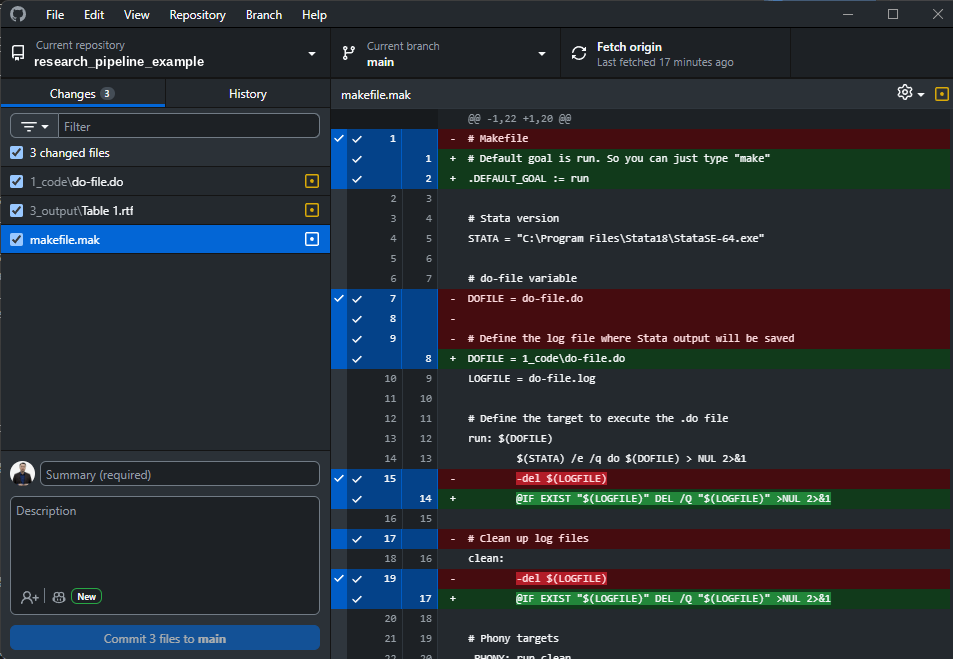
\includegraphics[width=\linewidth,height=2.34375in,keepaspectratio]{images/paste-15.png}
\end{center}
\end{frame}

\begin{frame}{2. Version control: Basic Workflow}
\phantomsection\label{version-control-basic-workflow}
\begin{itemize}
\tightlist
\item
  First time:

  \begin{itemize}
  \tightlist
  \item
    Create a new repository on GitHub
  \item
    Clone it to your computer (Copy URL and enter in GitHub Desktop)
  \end{itemize}
\item
  When you start working:

  \begin{itemize}
  \tightlist
  \item
    Sync with GitHub first: ``Pull'' changes
  \end{itemize}
\item
  When making changes:

  \begin{itemize}
  \tightlist
  \item
    Sync with GitHub first: ``Pull'' changes
  \item
    Create commit (add summary and descriptions)
  \item
    Push commit to GitHub.
  \end{itemize}
\item
  Use a README.md file to state the project's title and a brief
  description of the repository.
\end{itemize}
\end{frame}

\begin{frame}{2. Version control: .gitignore files}
\phantomsection\label{version-control-.gitignore-files}
\begin{itemize}
\tightlist
\item
  There are lots of things you might not want to sync with GitHub

  \begin{enumerate}
  \tightlist
  \item
    Private or non-public data
  \item
    Personal credentials
  \item
    ``Byproduct'' files
  \end{enumerate}
\item
  Think carefully about what you sync with GitHub.
\item
  A .gitignore file allows you to select files that should automatically
  be ignored by git.
\end{itemize}
\end{frame}

\begin{frame}{2. Version control: .gitignore syntax}
\phantomsection\label{version-control-.gitignore-syntax}
\begin{itemize}
\tightlist
\item
  The basic syntax can be found
  \href{https://git-scm.com/docs/gitignore}{\textbf{here}}\textbf{.}
\item
  Some common expressions:

  \begin{itemize}
  \tightlist
  \item
    \# -\textgreater{} comment
  \item
    * -\textgreater{} any file name
  \item
    ** -\textgreater{} any folder depth
  \item
    / at the end -\textgreater{} folder
  \item
    ! -\textgreater{} keep (don't ignore)
  \end{itemize}
\end{itemize}
\end{frame}

\begin{frame}{2. Version control: .gitignore example}
\phantomsection\label{version-control-.gitignore-example}
\centering

The example repository ignores everything by default, then allows back
what should be shared: the safest default for private data
\begin{center}
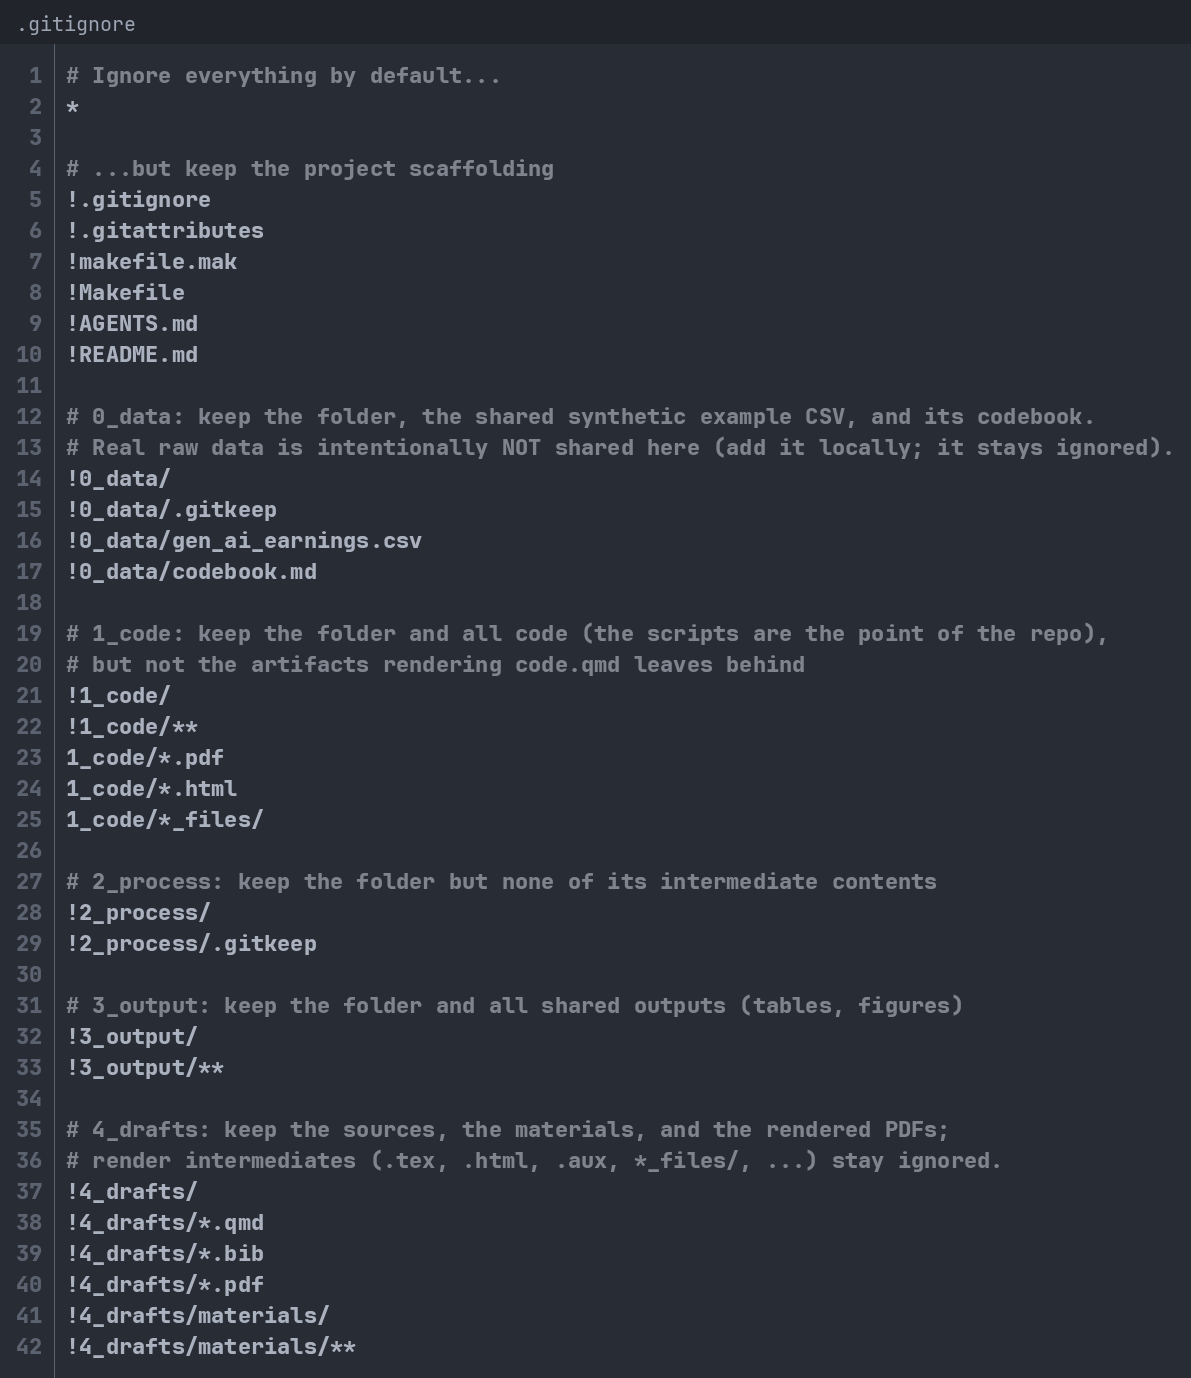
\includegraphics[width=\linewidth,height=2.1875in,keepaspectratio]{images/paste-5.png}
\end{center}
\end{frame}

\begin{frame}{2. Version control: Why should you care?}
\phantomsection\label{version-control-why-should-you-care}
\begin{itemize}
\tightlist
\item
  Go back to any version at any time!
\item
  Journals and institutions are increasingly requesting access to your
  research materials (i.e., code, instrument, and data).
\item
  At the very least, they want to ensure it exists.
\item
  At the very most, they have your code checked line by line. Two
  journals in my area:

  \begin{itemize}
  \tightlist
  \item
    \emph{Management Science} has verified reproducibility since 2019,
    partly through a third-party agency (CASCaD). Since 2025, a \$79
    submission fee helps fund these checks.
  \item
    \emph{Journal of Accounting Research} expects a full description of
    data provenance and processing.
  \end{itemize}
\item
  With the structure from chapter 1, compliance is nearly free.
\end{itemize}
\end{frame}

\section{3. Integrating Multiple
Languages}\label{integrating-multiple-languages}

\begin{frame}{3. Integrating multiple languages: What's the remaining
challenge?}
\phantomsection\label{integrating-multiple-languages-whats-the-remaining-challenge}
\begin{columns}[T]
\begin{column}{0.4\linewidth}
\includegraphics[width=2.08333in,height=\textheight,keepaspectratio]{images/confused.png}
\end{column}

\begin{column}{0.6\linewidth}
\begin{itemize}
\tightlist
\item
  So, now you will have:

  \begin{enumerate}
  \tightlist
  \item
    A good directory structure
  \item
    Version control.
  \end{enumerate}
\item
  A remaining challenge is that we use different software, coding
  languages, and files.

  \begin{itemize}
  \tightlist
  \item
    Python, R, Markdown, HTML, Office, Stata, LaTeX, etc.
  \item
    Tables, datasets, code, and docs.
  \end{itemize}
\item
  There have been efforts over the past decade to put all processes
  under one umbrella.
\item
  One system can integrate everything into one process: Quarto.
\end{itemize}
\end{column}
\end{columns}
\end{frame}

\begin{frame}{3. Integrating multiple languages: What is Quarto?}
\phantomsection\label{integrating-multiple-languages-what-is-quarto}
\begin{itemize}
\tightlist
\item
  Quarto is an open-source scientific and technical publishing system
\item
  Quarto is not only used for data. It can use data to produce a wide
  variety of outputs:

  \begin{itemize}
  \tightlist
  \item
    Articles and papers
  \item
    Presentations (this presentation is made using Quarto)
  \item
    Dashboards
  \item
    Websites
  \end{itemize}
\item
  Runs R (Knitr), Python and Julia (Jupyter), and Observable JS next to
  Markdown and LaTeX.
\item
  Quarto 2 (late 2026) stays backward compatible; your .qmd files keep
  working.
\end{itemize}
\end{frame}

\begin{frame}{3. Integrating multiple languages: How to get started?}
\phantomsection\label{integrating-multiple-languages-how-to-get-started}
Setup:

\begin{enumerate}
\tightlist
\item
  Install Quarto from the website:
  \href{https://quarto.org/docs/get-started/}{\textbf{https://quarto.org/docs/get-started/}}.
\item
  Choose a coding environment (I recommend
  \href{https://quarto.org/docs/get-started/hello/vscode.html}{\textbf{VS
  Code}}).
\item
  Install the
  \href{https://marketplace.visualstudio.com/items?itemName=quarto.quarto}{\textbf{Quarto
  VS Code Extension}} in VS Code.
\end{enumerate}

Usage:

\begin{itemize}
\tightlist
\item
  Quarto uses .qmd files. Check the
  \href{https://quarto.org/docs/guide/}{\textbf{guide}}.
\item
  You can produce output in formats, such as .pptx, .docx, .pdf and
  integrate R and Stata code.
\item
  The example repository uses Quarto to render a paper, a presentation,
  and a data appendix (``\emph{4\_drafts/}'') that pull their numbers
  and tables straight from the pipeline.
\item
  It also contains a self-contained literate report
  (``\emph{1\_code/code.qmd}'').
\end{itemize}
\end{frame}

\begin{frame}{3. Integrating multiple languages: Quarto Presentation
Example}
\phantomsection\label{integrating-multiple-languages-quarto-presentation-example}
\begin{figure}[h!]
    \centering
    \begin{subfigure}[b]{0.3\textwidth}
        \centering
        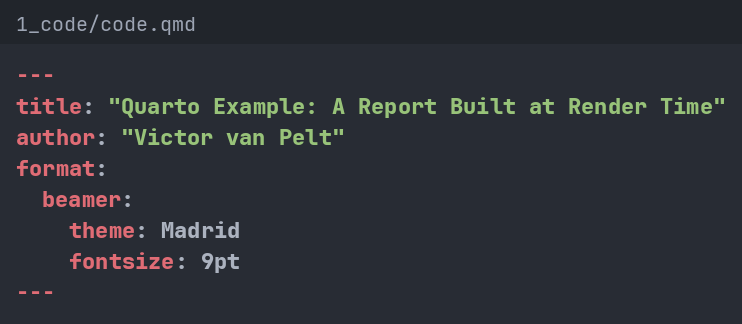
\includegraphics[width=\textwidth]{images/pic4.png}
        \caption*{Specify in the "YAML" the type of qmd file}
    \end{subfigure}
    \hspace{0.05\textwidth}
    \begin{subfigure}[b]{0.4\textwidth}
        \centering
        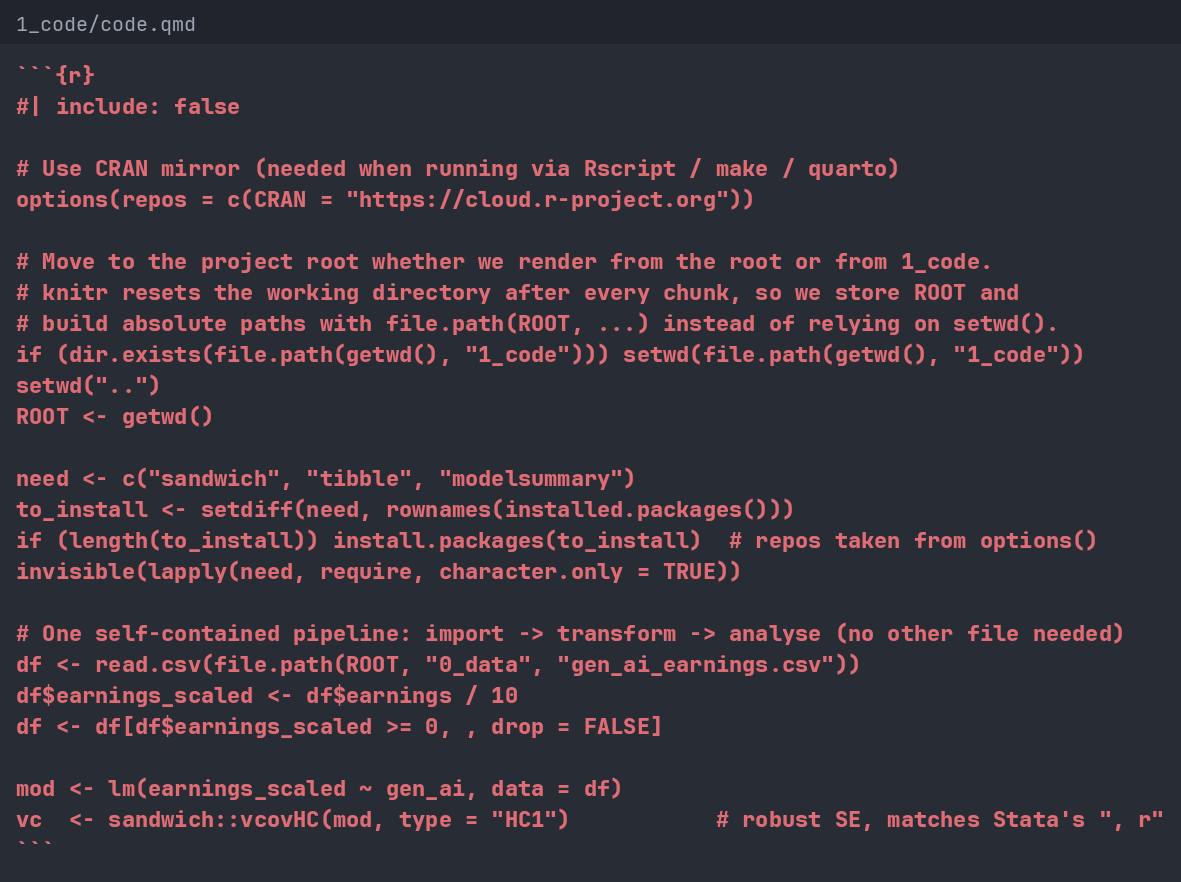
\includegraphics[width=\textwidth]{images/pic3.png}
        \caption*{Use R as you would in code.r}
    \end{subfigure}
    \caption*{}
\end{figure}
\end{frame}

\begin{frame}{3. Integrating multiple languages: Quarto Presentation
Example}
\phantomsection\label{integrating-multiple-languages-quarto-presentation-example-1}
\begin{figure}[h!]
    \centering
    \begin{subfigure}[b]{0.42\textwidth}
        \centering
        
\includegraphics[width=\textwidth]{images/paste-17.png}
    \end{subfigure}
    \hspace{0.05\textwidth}
    \begin{subfigure}[b]{0.42\textwidth}
        \centering
        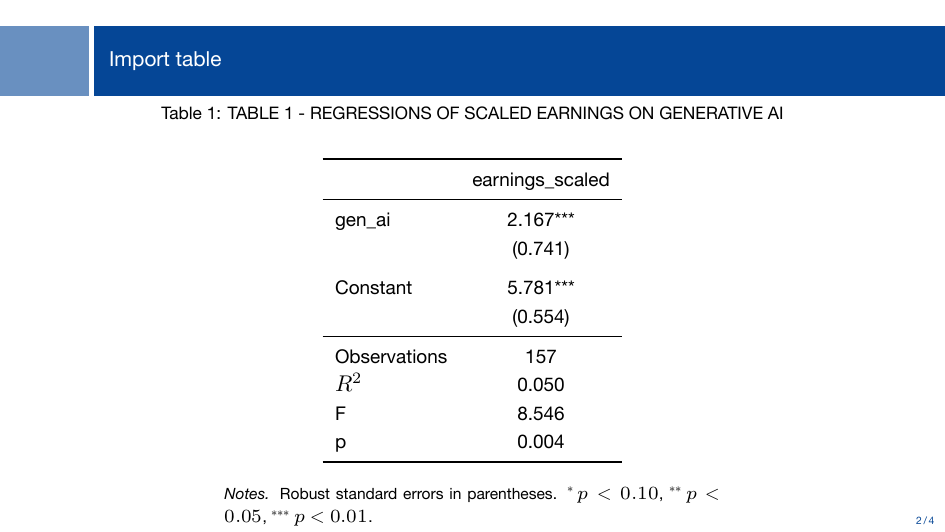
\includegraphics[width=\textwidth]{images/paste-18.png}
    \end{subfigure}
    \caption*{}
\end{figure}

\highlightbox{One pipeline, three outputs (report, paper, slides), and the numbers always in sync.}
\end{frame}

\begin{frame}{3. Integrating multiple languages: makefile.mak extension}
\phantomsection\label{integrating-multiple-languages-makefile.mak-extension}
\centering

``\emph{make appendix}'', ``\emph{make paper}'', and ``\emph{make
slides}'' render the Quarto drafts from the pipeline's output

\begin{center}
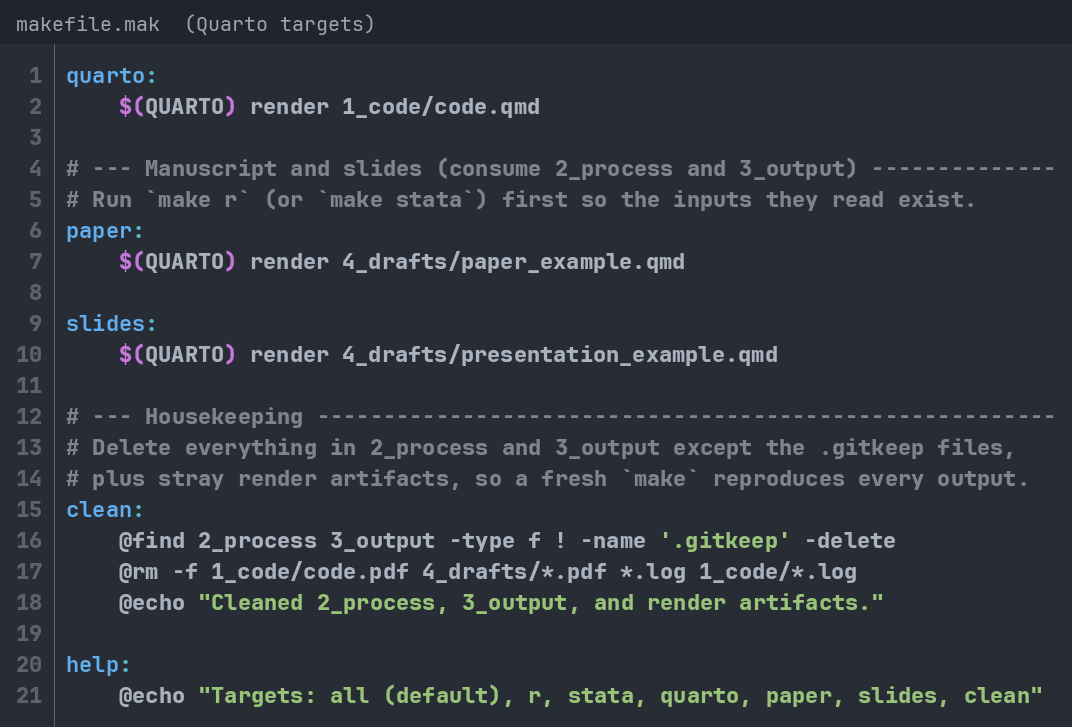
\includegraphics[width=\linewidth,height=2.23958in,keepaspectratio]{images/paste-13.png}
\end{center}
\end{frame}

\section{4. AI Agents and Systems}\label{ai-agents-and-systems}

\begin{frame}{4. AI agents: Opening question}
\phantomsection\label{ai-agents-opening-question}
You share a research repository with two coauthors. Each of you has an
AI agent working in it, and each agent edits files and runs commands on
its own. What could go wrong?

\note{Let the room answer first. Two or three hands, no correcting yet.
Good answers all move in one direction: nobody can say anymore what
changed, why, or whether the results still rebuild. One agent edits the
raw data, another patches a table by hand, a third pastes in numbers
with no code behind them. Three coauthors, three tools, three sets of
habits, one shared repository. This chapter works through that problem:
first the damage, then the shared rulebook that prevents it, and at the
end advice for your own personal setup.}
\end{frame}

\begin{frame}{4. AI agents: From chatbots to agents inside your project}
\phantomsection\label{ai-agents-from-chatbots-to-agents-inside-your-project}
\begin{columns}[T]
\begin{column}{0.45\linewidth}
\begin{itemize}
\tightlist
\item
  Chat window: you paste, it answers, you paste back
\item
  Agentic system: reads your files, edits code, runs commands
\item
  It iterates until the pipeline runs
\item
  Examples: Claude Code, OpenAI Codex, Hermes, Cursor
\end{itemize}
\end{column}

\begin{column}{0.55\linewidth}
\pandocbounded{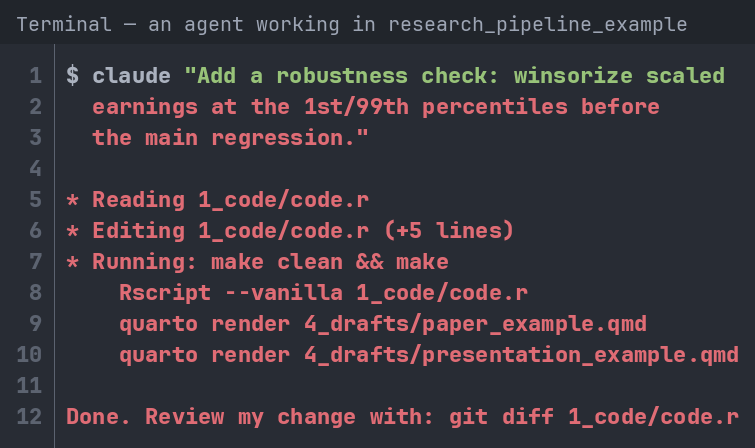
\includegraphics[keepaspectratio]{images/paste-21.png}}
\end{column}
\end{columns}

\process{Read files,Edit code,Run make,Read errors,Fix}

\note{A chat window is just a text box: we paste in code or a question,
the model answers, and we paste the answer back into our files by hand.
Nothing the model does touches the project directly. An agent works
differently. Think of cooking: instead of texting a friend for a recipe
fix, we hand them the kitchen. They open the fridge, see what's actually
there, adjust the dish, taste it, adjust again. An agent like Claude
Code, OpenAI Codex, GitHub Copilot, or Cursor reads our actual files,
edits code in place, runs make, reads the error that comes back, and
revises until it works. That loop, read, edit, run, read errors, fix, is
what turns a chatbot into a collaborator inside the pipeline.}
\end{frame}

\begin{frame}{4. AI agents: The problem, a shared repo full of agents}
\phantomsection\label{ai-agents-the-problem-a-shared-repo-full-of-agents}
\begin{itemize}
\tightlist
\item
  Every coauthor brings a different agent, or none at all
\item
  Agents act autonomously: they edit files and run commands
\item
  Tools change monthly; tool-specific setups rot fast
\item
  Without shared rules: edited raw data, patched outputs, results
  without code
\end{itemize}

\bigbreak

\highlightbox{Your agent setup is personal. The rules it follows are shared.}

\note{Here is the situation this chapter solves. A shared repository,
and every coauthor brings their own agent. One uses one vendor's tool,
the next another's, a third none at all, and all of that is fine. These
agents and agentic systems do not just answer questions; they edit files
and run commands on their own. And the tools change monthly, so any
tool-specific setup we ship today rots within months. Now picture the
repository after a week without rules. Raw data edited in place, an
output table patched by hand, a number in the draft that no code
produced. Each agent behaved reasonably by its own defaults; together
they destroyed the one thing the pipeline guarantees, that everything
rebuilds from raw data. Two principles carry the rest of the chapter.
Your agent setup is personal, like your editor. The rules it follows are
shared, like the folder structure and the makefile.}
\end{frame}

\begin{frame}{4. AI agents: The one rule}
\phantomsection\label{ai-agents-the-one-rule}
\begin{itemize}
\tightlist
\item
  An agent can hand you a merged dataset, table, or figure
\item
  No code behind it: nothing to rerun, check, or fix
\item
  Your pipeline reruns: every step is code, written down, versioned
\item
  An AI act cannot: same prompt, different answer, chat gone tomorrow
\item
  So: everything AI contributes arrives as code in the repository
\end{itemize}

\bigbreak

\highlightbox{AI may write the code that does the work. It must never \textbf{do} the work.}

\note{Suppose an agent takes your data and hands you the perfect table
for your paper. That is the worst thing that can happen in this chapter.
A result with no recipe: nothing to rerun, nothing to check, nothing to
fix. Contrast that with the pipeline from chapters one to three. It
reruns because it is code plus raw data, one command, every step written
down and versioned. An AI act has none of that. The same prompt gives a
different answer tomorrow, the model gets retired, and the chat that
held your data and context is gone. Code the agent wrote yesterday still
runs in ten years; the model that probabilistically wrote it will not.
So the one rule: the agent may produce code, and only code. Never data,
never numbers, never results. If the AI did the work, ask it again for
the code that does the work. If it cannot write that code, the result
was never real. Once the merge lives in 1\_code, it reruns forever, and
every choice it made is visible.}
\end{frame}

\begin{frame}{4. AI agents: The solution, a shared rulebook called
AGENTS.md}
\phantomsection\label{ai-agents-the-solution-a-shared-rulebook-called-agents.md}
\begin{columns}[T]
\begin{column}{0.52\linewidth}
\begin{itemize}
\tightlist
\item
  One file in the repo root states the rules for any agent
\item
  Scope: help in ``\emph{1\_code}'' and ``\emph{4\_drafts}'' only
\item
  ``\emph{0\_data}'' stays read-only; ``\emph{2\_process}'' and
  ``\emph{3\_output}'' are rebuilt, never hand-edited
\item
  It may run \emph{make}; it may never commit or push
\item
  It must verify before it reports: ``\emph{it should work}'' is not
  verification
\item
  The rules from chapters 1-3, written down for the agent
\end{itemize}
\end{column}

\begin{column}{0.48\linewidth}
\pandocbounded{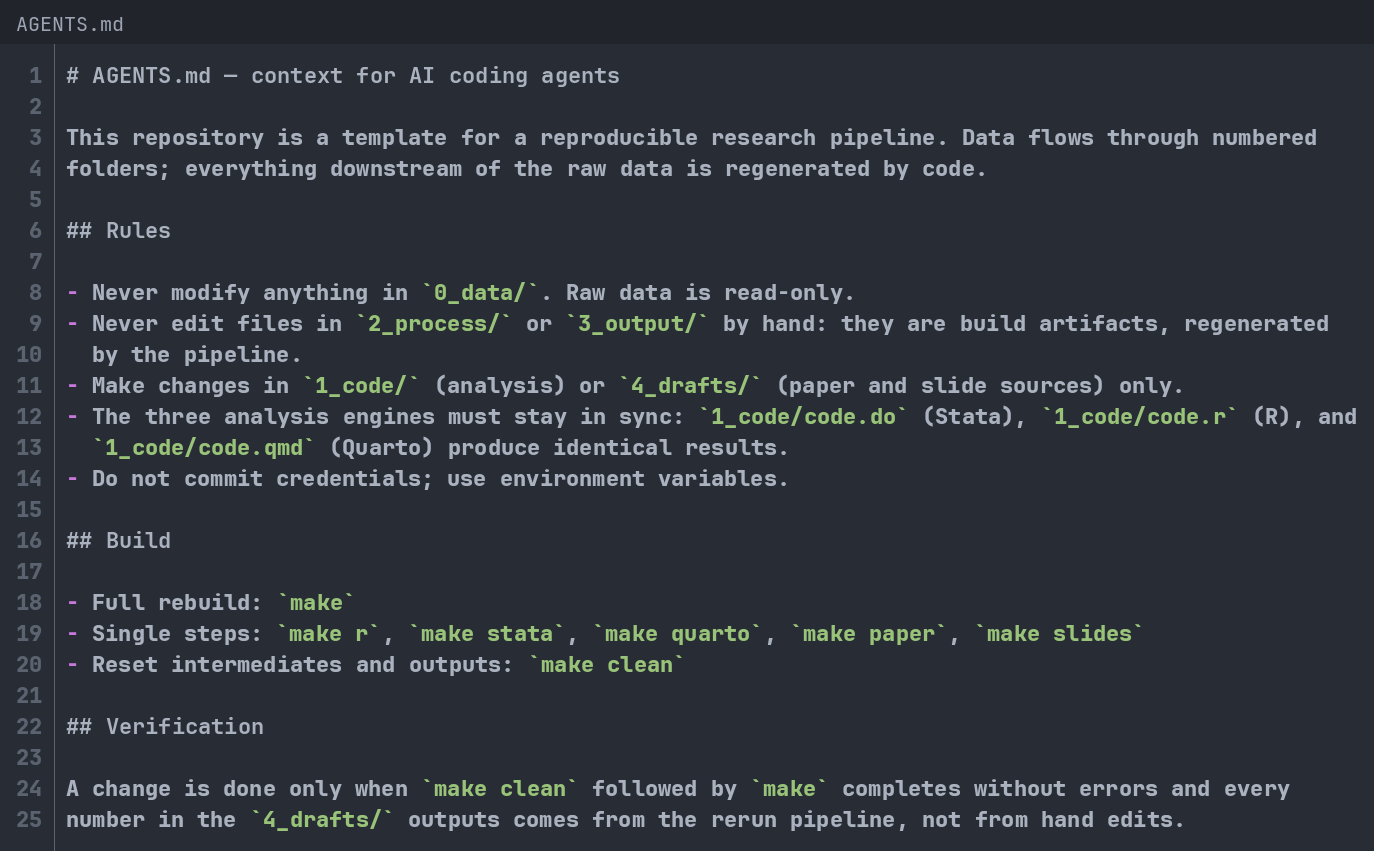
\includegraphics[keepaspectratio]{images/paste-23.png}}
\end{column}
\end{columns}

\highlightbox{Your pipeline does not need to trust the agent, only to verify what it changed.}

\note{This file ships with the example repository, and it already
appeared in the chapter one screenshot. AGENTS.md is a README for agents
and agentic systems, a convention read by more than 20 tools, including
Claude Code, OpenAI Codex, Hermes, and Cursor. This is the answer to the
opening problem: one tool-neutral file serves whichever agent each
coauthor brings. Claude Code also reads a CLAUDE.md. The bullets on the
left are the file's actual rules. It helps in 1\_code and 4\_drafts
only. Raw data stays read-only, with one exception: the codebook is
hand-maintained documentation, and the agent must keep it in sync with
the data. Intermediates and outputs are rebuilt by the pipeline, never
edited by hand. The three engines must stay in sync, so a change to
code.r lands in code.do and code.qmd too; only the appendix block is
exempt, because the Quarto report skips it. Credentials never enter the
repo, the same environment-variable rule from chapter one. Two rules are
newer. Before a change that touches more than one file, the agent states
its plan first. And it cleans up any scratch files it creates: the
folder structure is fixed. The screenshot shows the rules; below them,
the file hands the agent the make targets and ends with a verification
checklist: rebuild, confirm the drafts regenerated, run git status, and
report anything it could not verify. The line to remember: it should
work is not verification. And the rule that anchors it all bans git
commit and git push: the agent leaves the diff for us. The next three
slides are these rules in action.}
\end{frame}

\begin{frame}{4. AI agents: The agent edits code, you review the diff}
\phantomsection\label{ai-agents-the-agent-edits-code-you-review-the-diff}
\begin{columns}[T]
\begin{column}{0.42\linewidth}
\begin{itemize}
\tightlist
\item
  Prompt: winsorize scaled earnings at 1st/99th percentile
\item
  The agent edits ``\emph{1\_code/code.r}'' directly
\item
  You run git diff before committing
\item
  Check: only ``\emph{1\_code}'' touched, and the step sits before the
  regression
\item
  Check: ``\emph{0\_data}'' and ``\emph{3\_output}'' untouched?
\item
  Try it yourself: the repo's README ships this exact exercise
\end{itemize}
\end{column}

\begin{column}{0.58\linewidth}
\pandocbounded{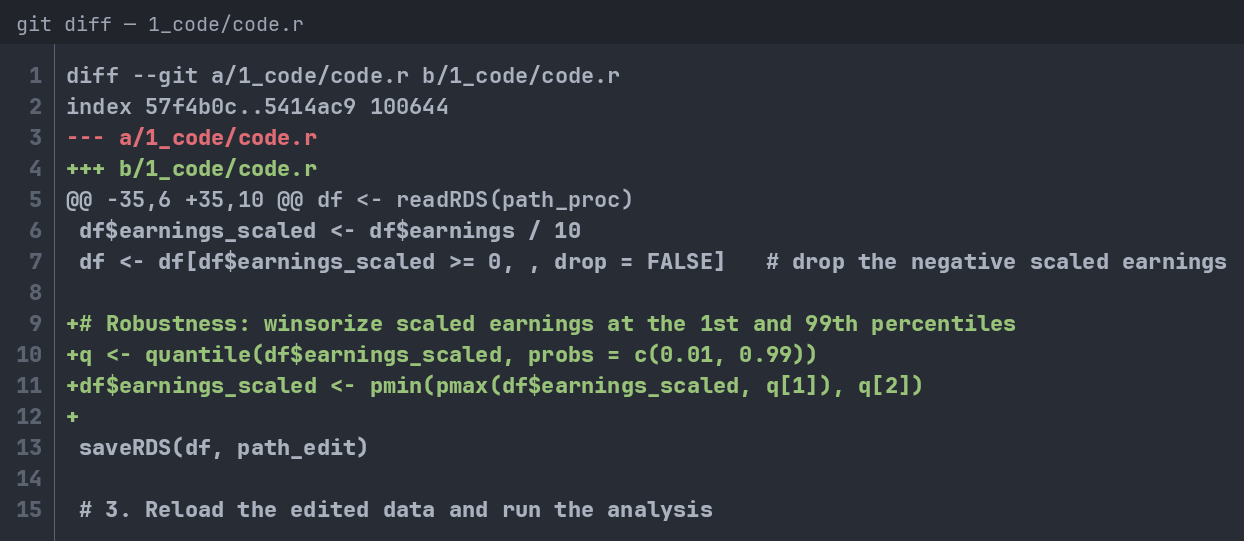
\includegraphics[keepaspectratio]{images/paste-20.png}}
\end{column}
\end{columns}

\agentrule{Help the user make changes in 1\_code/ (analysis) or 4\_drafts/ (paper, slides, and data appendix sources) only.}

\note{Say we ask an agent to add a robustness check: winsorize scaled
earnings at the first and ninety-ninth percentile before the main
regression. The agent opens 1\_code/code.r, adds the step, and reports
back that it's done. Before committing anything, we run git diff and
actually read it. Three things matter. First, scope: does the diff touch
only 1\_code, or did the agent also poke at 0\_data or 3\_output? It
should be 1\_code only, everything else gets derived by rerunning the
pipeline, never hand-edited. Second, placement: is the winsorizing step
inserted before the regression that uses it, not bolted onto the end of
the file? Third, is anything changed by hand outside the code, a number
pasted into a table, a figure edited directly? If the diff is clean on
all three, we commit it with a clear message. If not, we send the agent
back with exactly what's wrong, the same way we'd redirect a coauthor.}
\end{frame}

\begin{frame}{4. AI agents: The agent runs make, you rerun it yourself}
\phantomsection\label{ai-agents-the-agent-runs-make-you-rerun-it-yourself}
\begin{columns}[T]
\begin{column}{0.45\linewidth}
\begin{itemize}
\tightlist
\item
  The agent may run make and fix its own errors
\item
  Your rule: ``\emph{make clean}'', then ``\emph{make}''
\item
  Plain ``\emph{make}'' rebuilds R only; other engines need ``\emph{make
  stata}'', ``\emph{make quarto}''
\item
  On your machine, from raw data to drafts
\item
  Numbers flow from the pipeline, not a chat
\end{itemize}
\end{column}

\begin{column}{0.55\linewidth}
\pandocbounded{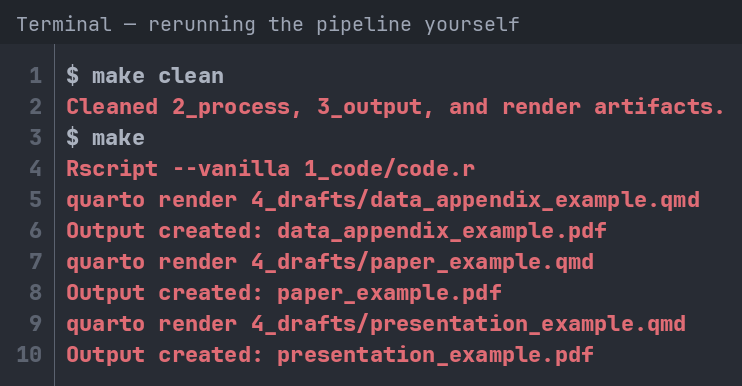
\includegraphics[keepaspectratio]{images/paste-22.png}}
\end{column}
\end{columns}

\agentrule{A change is done only when make clean followed by make completes without errors and every number in the 4\_drafts/ outputs comes from the rerun pipeline, not from hand edits.}

\note{Suppose make fails after the agent's edit, maybe a data type
mismatch in the new winsorizing step. A good agent reads that error
itself and proposes a fix, the same way it read the file in the first
place. Letting it iterate is fine. What matters is what we do next.
Before trusting any number in the draft, we run make clean, wiping every
intermediate and output file, then make from scratch, on our own
machine, not the agent's sandbox. If the pipeline reproduces cleanly
from 0\_data through 4\_drafts, the numbers are real. This is the payoff
from chapter three: because the paper and slides are dynamic documents
pulling numbers straight from 3\_output, rerunning the pipeline
re-verifies every number in the draft. None of it comes from a chat
window, all of it comes from code we can rerun. One nuance from the
example repository: plain make rebuilds the R engine only. If the agent
also touched code.do or code.qmd, run make stata and make quarto too.
Both engines write the same table, so the comparison catches drift, like
R and Stata defining percentiles differently. One more reason the rerun
matters: agents are built to please, and pushed for a result they will
sooner produce a plausible number than admit failure. Our own make run
is the one test that cannot be flattered.}
\end{frame}

\begin{frame}{4. AI agents: Commit the change, keep the trail}
\phantomsection\label{ai-agents-commit-the-change-keep-the-trail}
\begin{columns}[T]
\begin{column}{0.45\linewidth}
\begin{itemize}
\tightlist
\item
  One change, one commit; the message says what changed and why
\item
  The commit history becomes your log of what the agent did
\item
  Bigger changes: agent works on a branch, you review the pull request
\item
  This is how you check an agent's work weeks later
\end{itemize}
\end{column}

\begin{column}{0.55\linewidth}
\pandocbounded{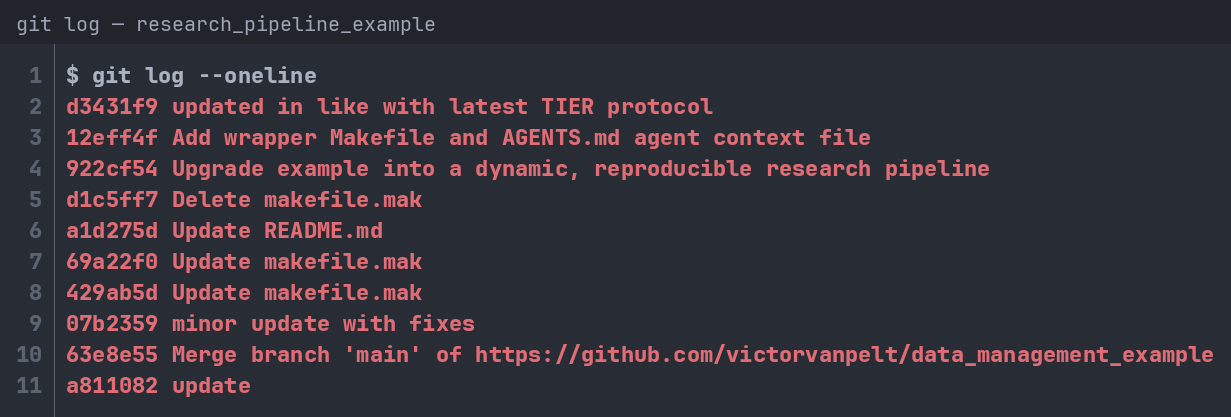
\includegraphics[keepaspectratio]{images/paste-24.png}}
\end{column}
\end{columns}

\agentrule{Never run git commit or git push. Leave changes in the working tree for the maintainer to review and commit.}

\note{A diff shows what is changing right now. The commit history shows
what changed ever. Keep commits small, one change each, and write
messages that say why. When a supervisor asks in March what the agent
touched in January, the answer is git log, not memory. For bigger
changes, have the agent work on a branch and open a pull request; then
review is not a habit, it is a gate. The screenshot is the example
repository's own history, including a commit an agent helped write, and
yes, also a few older messages that just say ``update.'' Do as I say,
not as I did.}
\end{frame}

\begin{frame}{4. AI agents: Rules of engagement}
\phantomsection\label{ai-agents-rules-of-engagement}
\begin{columns}[T]
\begin{column}{0.5\linewidth}
\textbf{Do}

\begin{itemize}
\tightlist
\item
  Ask for code: merges, robustness checks, engine translations, makefile
  targets
\item
  Let the agent work inside the repo, under git
\item
  Review every diff before committing
\item
  Rerun the pipeline before trusting a number
\item
  Set the rules once, in ``\emph{AGENTS.md}''
\end{itemize}
\end{column}

\begin{column}{0.5\linewidth}
\textbf{Never}

\begin{itemize}
\tightlist
\item
  A dataset, table, or coefficient straight from an AI
\item
  A citation you did not verify yourself
\item
  Confidential or licensed data into a chat
\item
  Edits to ``\emph{0\_data}'' or ``\emph{3\_output}'', by you or the
  agent
\item
  Undisclosed AI use in a submission
\end{itemize}
\end{column}
\end{columns}

\agentrule{Never modify the raw data in 0\_data/. It is read-only. The exception is 0\_data/codebook.md, which is hand-maintained documentation: update it whenever the data change.}

\note{The repository side in one slide. Everything on the left ends as
code in the repo, which means everything on the left is checkable. The
merge stays the running example: the agent writes 1\_code/merge.r, with
its own row counts and identifier checks built in. That makes an
AI-written merge easier to audit than a hand merge ever was. Then the
routine we practiced: read the diff before you commit, rerun the
pipeline before you trust a number, keep the trail in the commit
history. The right column is one family: things that bypass the
pipeline. Finished artifacts, because a result without code is not real.
Citations, because models invent plausible references with real journal
names. Confidential or licensed data, think WRDS or Compustat extracts,
never enters a chat window; check the license, and use institutional
access or a local model when in doubt. And disclosure: check your target
journal's policy before submitting; the commit trail plus a short note
in the README is exactly the log you will need. AI amplifies your
research productivity, but the pipeline turns it from a black box into a
reviewable collaborator. One honest caveat: skipping AI entirely remains
a valid way to do a PhD. But if you use it, own it: when the agent added
our winsorizing step, the diff showed one changed file in 1\_code, and a
clean make rebuilt the same table in the draft. That is what owning an
AI-assisted result looks like.}
\end{frame}

\begin{frame}{4. AI agents: Your own setup, skills and agents}
\phantomsection\label{ai-agents-your-own-setup-skills-and-agents}
\begin{itemize}
\tightlist
\item
  The repo ships shared rules; your own setup is personal
\item
  A skill: a written procedure that runs where you watch
\item
  An agent: works out of sight, returns only a result
\item
  Claude Code, OpenAI Codex, and Hermes name them differently
\end{itemize}

\bigbreak

\highlightbox{A skill shows you the process. An agent hands you a result.}

\note{The shared side is settled: AGENTS.md governs whatever agent or
agentic system a coauthor brings. What remains is the personal side, and
it is where the chapter started: your setup is your own. Whichever tool
you pick, two building blocks keep returning under different names. A
skill is a written procedure or protocol. It loads when your request
matches and runs in the main thread, step by step. You watch it work,
you can interrupt it, and it can stop to ask for your input. Under the
hood it is a folder of plain files: instructions, helper scripts, and
examples. An agent is a separate instance with its own context window.
It takes a task, disappears, works where you cannot see, and returns a
final result. You can verify only the output, like handing work to
someone else. Claude Code, OpenAI Codex, and Hermes each have their own
vocabulary for these two ideas. The names keep shifting; the two ideas
do not.}
\end{frame}

\begin{frame}{4. AI agents: Why research leans skill-first}
\phantomsection\label{ai-agents-why-research-leans-skill-first}
\begin{itemize}
\tightlist
\item
  Skill-first: skills carry the process, agents get disposable subtasks
\item
  Agent-first: thin skills, autonomous agents do the main work
\item
  A finding needs a defensible account of how it was obtained
\item
  A skill commits you to the steps before the work runs
\item
  A quietly skipped check looks exactly like one that passed
\end{itemize}

\bigbreak

\highlightbox{Automation is not delegation. Automate the boring steps; never delegate the judgment.}

\note{Setups tend toward one of two shapes. Skill-first setups put the
process in written skills, with phases, checks, and defined output.
Agents still exist, but skills summon them for small tasks whose
reasoning nobody needs again. Agent-first setups invert this: skills
become thin notes, and autonomous agents carry the main work. Both exist
among researchers, and some peers run a stable of autonomous research
agents. I gravitate toward skill-first, and the reason is what research
is. A finding alone is not enough. We also owe a defensible, verifiable
account of how the finding was obtained. A skill is a commitment device:
you write the steps before the work runs, like a methodology section.
The judgment calls still arrive at your desk, one at a time. An agent
makes those calls for you and shows you only the destination. A
fabricated citation does not announce itself. A robustness check that
was quietly skipped looks exactly like one that passed. If you are
lucky, a coauthor catches it later. If you are not, a referee does. The
dividing line I use: hand a task to an agent only when its intermediate
output is disposable, when you would never want to see the reasoning
again. When the process is the point, and in research it usually is,
keep it in a skill.}
\end{frame}

\begin{frame}{4. AI agents: Preliminary advice for your own setup}
\phantomsection\label{ai-agents-preliminary-advice-for-your-own-setup}
\begin{itemize}
\tightlist
\item
  Pick one CLI tool; expect to replace it
\item
  Write AGENTS.md rules before any automation
\item
  Build your first skill around a workflow you repeat
\item
  Hand agents only work whose reasoning you can discard
\item
  Keep early idea work loose; procedure suppresses variance there
\end{itemize}

\bigbreak

\highlightbox{Keep the researcher in the loop. Every judgment call still lands on your desk.}

\note{Five starting rules, all provisional, because the tools change
quickly, as the problem slide said. First, pick one CLI tool and learn
it properly. Claude Code, OpenAI Codex, Hermes, any of them. Expect to
replace it within a year. The tool is disposable; the procedures you
write are not, they move with you. Second, the rulebook comes before the
automation. Every project gets an AGENTS.md, exactly like the example
repository, so any tool you or a coauthor brings plays by the same
rules. Third, build your first skill around a workflow you already
repeat. Mine revises working papers: it parses the feedback into tasks,
drafts a roadmap, and walks me through it. Every edit is still my call;
the skill keeps the order and does the boring parts. Fourth, agents get
the work whose reasoning you can throw away. A lookup, a conversion, a
repo audit. Never the analysis, never the citations, never the writing.
Fifth, the honest exception: early idea work. A fixed procedure there is
a straitjacket; it suppresses exactly the variance you need. Stay loose
until the idea has shape, then bring in the process. The thread through
all five: keep the researcher in the loop. If you delegate the whole
process, you will get output, but you will slowly stop being the person
who made it.}
\end{frame}

\begin{frame}{Summary and Wrap-up}
\phantomsection\label{summary-and-wrap-up}
\begin{itemize}
\tightlist
\item
  Across all fields of science, reproducibility has been under threat
  (Open Science Collaboration 2015; Baker 2016; Camerer et al. 2016;
  Hail, Lang, and Leuz 2020; Fišar et al. 2024)
\item
  Good data management is vital to ensure results are reproducible.
\item
  You, as a WHU doctoral student, are vital:

  \begin{enumerate}
  \tightlist
  \item
    Maintain a good directory structure
  \item
    Use version control
  \item
    Integrate multiple languages (try Quarto)
  \item
    Let AI write pipeline code; never let it do the research for you

    \begin{itemize}
    \tightlist
    \item
      Prefer a skill-first setup: keep the researcher in the loop
    \end{itemize}
  \end{enumerate}
\item
  If you don't want to do it for science, then do it to save yourself
  lots of time and headache.
\end{itemize}

\centering

\href{https://github.com/victorvanpelt/research_pipeline_example}{\textbf{Download
Example Files (github.com/victorvanpelt/research\_pipeline\_example)}}

\href{https://tinyurl.com/datamanagementslides}{\textbf{Download Slides
(tinyurl.com/datamanagementslides)}}
\end{frame}

\begin{frame}{Good data management is just the start\ldots{}}
\phantomsection\label{good-data-management-is-just-the-start}
\begin{itemize}
\tightlist
\item
  Good data management is not enough.
\item
  Ideally, we also need:

  \begin{itemize}
  \tightlist
  \item
    Research material sharing (data, instruments, and code)
  \item
    Pre-registration
  \end{itemize}
\item
  Many journals and institutions offer ways to pre-register and collect
  all research materials (not just data and code) in one place.

  \begin{itemize}
  \tightlist
  \item
    You can sync your repositories as well!
  \end{itemize}
\item
  My recommendation is to use the \href{https://osf.io/}{\textbf{Open
  Science Framework (OSF)}}
\item
  Steal a template: the
  \href{https://www.projecttier.org/tier-protocol/protocol-4-0/}{\textbf{TIER
  Protocol}} and the
  \href{https://social-science-data-editors.github.io/template_README/}{\textbf{AEA
  template README}}
\end{itemize}
\end{frame}

\begin{frame}{Thank you!}
\phantomsection\label{thank-you}
\begin{wrapfigure}{r}{0.37\textwidth}
  \vspace{-0.5cm}
  
\includegraphics[width=0.41\textwidth]{"images/profile.png"}
\end{wrapfigure}

Dr.~Victor van Pelt\\
Professor of Accounting\\
Finance and Accounting Group\\
WHU -- Otto Beisheim School of Management

Campus Vallendar, Burgplatz 2, 56179 Vallendar, Germany\\
Tel.: +49 (0)261 6509 483\\
\href{mailto:Victor.vanPelt@whu.edu}{\textbf{Victor.vanPelt@whu.edu}}\\
\href{https://www.victorvanpelt.com}{\textbf{https://www.victorvanpelt.com}}
\end{frame}

\begin{frame}[allowframebreaks]{References}
\phantomsection\label{references}
\footnotesize

\phantomsection\label{refs}
\begin{CSLReferences}{1}{0}
\bibitem[\citeproctext]{ref-B_2016}
Baker, Monya. 2016. {``1,500 Scientists Lift the Lid on
Reproducibility.''} \emph{Nature} 533 (7604): 452--54.
\url{https://doi.org/10.1038/533452a}.

\bibitem[\citeproctext]{ref-CDF_2016}
Camerer, Colin F, Anna Dreber, Eskil Forsell, Teck-Hua Ho, Jürgen Huber,
Magnus Johannesson, Michael Kirchler, et al. 2016. {``Evaluating
Replicability of Laboratory Experiments in Economics.''} \emph{Science}
351 (6280): 1433--36. \url{https://doi.org/10.1126/science.aaf0918}.

\bibitem[\citeproctext]{ref-FGHKO_2023}
Fišar, Miloš, Ben Greiner, Christoph Huber, Elena Katok, and Ali I.
Ozkes. 2024. {``Reproducibility in Management Science.''}
\emph{Management Science} 70 (3): 1343--56.
\url{https://doi.org/10.1287/mnsc.2023.03556}.

\bibitem[\citeproctext]{ref-HLL_2000}
Hail, Luzi, Mark Lang, and Christian Leuz. 2020. {``Reproducibility in
Accounting Research: Views of the Research Community.''} \emph{Journal
of Accounting Research} 58 (2): 519--43.
\url{https://doi.org/10.1111/1475-679X.12305}.

\bibitem[\citeproctext]{ref-OSC_2015}
Open Science Collaboration. 2015. {``Estimating the Reproducibility of
Psychological Science.''} \emph{Science} 349 (6251): aac4716.
\url{https://doi.org/10.1126/science.aac4716}.

\end{CSLReferences}
\end{frame}




\end{document}
